
%region : INTELLIJ
\section{Conociendo \textit{IntelliJ}} 
  \subsection{Creando un proyecto}
    El primer paso para utilizar \textit{IntelliJ} es abrirlo 
    \begin{center}
      amazing
    \end{center}
    esto puede tomar algunos minutos dado que el \textit{IDE} ocupa muchos recursos.

    \begin{figure}[ht!]
      \centering
      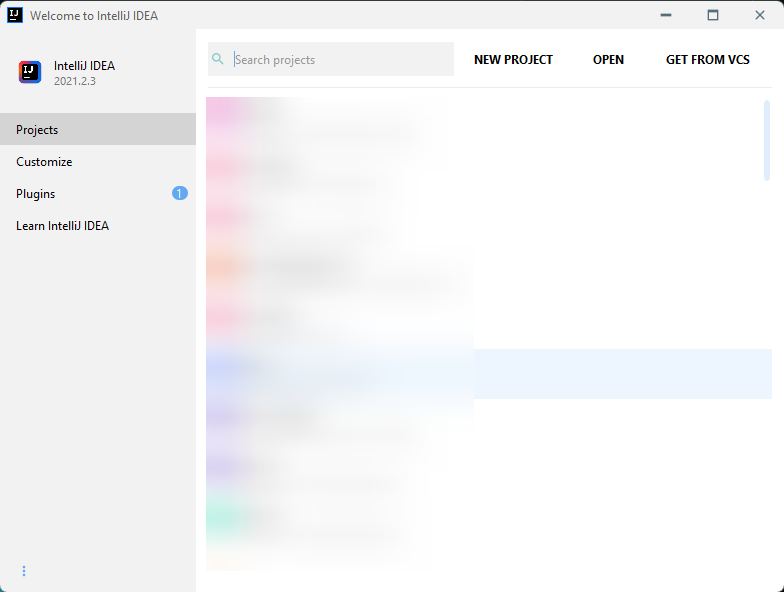
\includegraphics[width=0.5\textwidth]{img/Por_algo_se_empieza/idea64_HkClRzeuYD.png}
      \caption{Ventana inicial de \textit{IntelliJ}.}
      \label{fig:intellij-landing}
    \end{figure}
    
    Una vez abierto debieran ver una ventana similar a la de la figura \ref{fig:intellij-landing}.
    Aquí deberán seleccionar la opción \enquote{\textit{New Project}}.

    \begin{figure}[ht!]
      \centering
      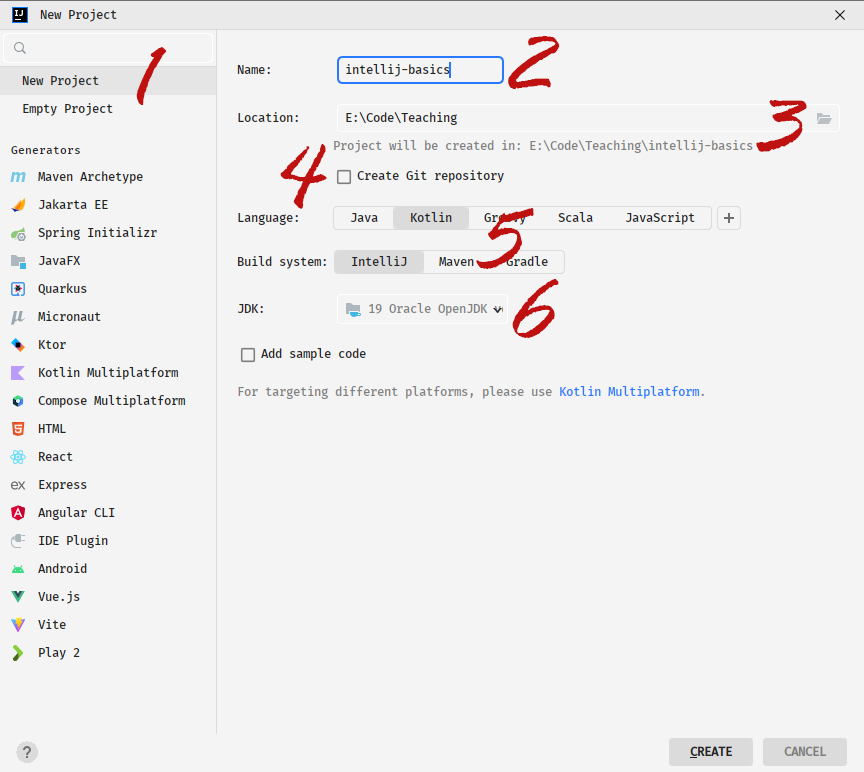
\includegraphics[width=0.7\textwidth]{img/Por_algo_se_empieza/idea64_new_project_1.png}
      \caption{Ventana de creación de proyectos}
      \label{fig:intellij-new-project-1}
    \end{figure}

    Luego deberíamos estar en la ventana principal de creación de proyectos (figura 
    \ref{fig:intellij-new-project-1}), aquí tendremos muchas opciones disponibles pero en este
    libro las ignoraremos y sólo le pondremos atención a proyectos de \textit{Kotlin}.
    En esta ventana, primero seleccionaremos la opción \textit{New Project} (1), ahí tendremos la
    opción de nombrar nuestro proyecto (2), pongámosle \enquote{intellij-basics}.
    Luego, colocamos la ubicación donde queremos que se cree el proyecto (3), en este caso se 
    guardará en \mintinline{text}{E:\Code\Teaching} (donde se creará una sub-carpeta con el nombre
    del proyecto).
    Por ahora, desmarquemos la opción \textit{Create Git repository} (4) ya que no vamos a 
    utilizarlo todavía.
    Lo siguiente es seleccionar el lenguaje y \textit{build system} que vamos a utilizar (5), en
    este caso seleccionaremos \textit{Kotlin} e \textit{IntelliJ} respectivamente, por ahora no nos
    vamos a detener en lo que es un \textit{build system}.
    Finalmente, debemos seleccionar la distribución de \textit{JDK} que vamos a utilizar (6), en
    este caso seleccionaremos la última versión de \textit{JDK} disponible (19 en el ejemplo).

    Con esto podemos darle \textit{Create} al proyecto, esperamos unos segundos para que se cocine
    y listo, ya tenemos nuestro primer proyecto en \textit{IntelliJ}.

  \subsection{Trabajando con \textit{IntelliJ}}
    \label{sec:intellij-work}

    Hasta ahora hemos utilizado la terminal para programar en kotlin, esto es bastante útil pero
    \textit{IntelliJ} nos ofrece muchas más herramientas para programar.
    La primera que veremos es la \idxit{consola REPL} (\textit{Read-Eval-Print-Loop}), esto es
    similar a utilizar \textit{Kotlin} en la terminal pero con muchas más herramientas.

    \begin{figure}[ht!]
      \centering
      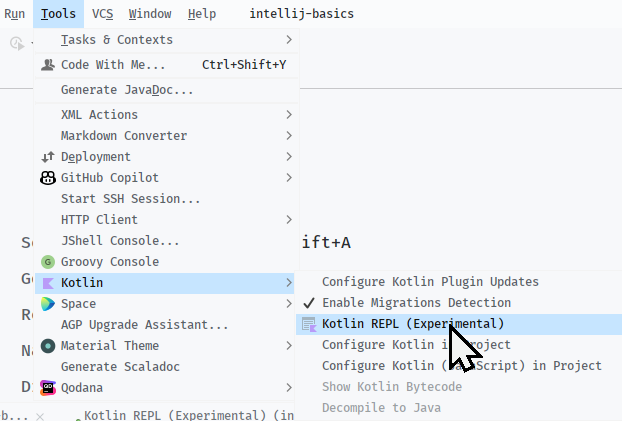
\includegraphics[width=0.5\textwidth]{img/Por_algo_se_empieza/idea64_tools_repl.png}
      \caption{ubicación de la \textit{consola REPL} en \textit{IntelliJ}.}
      \label{fig:tools-repl}
    \end{figure}

    Para acceder a la consola REPL, debemos ir a la sección \enquote{Tools} de la barra de 
    herramientas, ir a la opción \enquote{Kotlin} y seleccionar la opción \enquote{\textit{Kotlin REPL 
    (Experimental)}} (figura \ref{fig:tools-repl}).
    
    \begin{tcolorbox}[enhanced, breakable, title=\textit{Search Everywere}]
      Otra forma de acceder a la \textit{consola REPL} es utilizando la herramienta \idxit{Search
      Everywhere} (figura \ref{fig:idea64-search-everywhere}), esta herramienta nos permite buscar
      casi todo en \textit{IntelliJ} y nos permite acceder a herramientas y archivos de manera 
      rápida.
      Para utilizarla, debemos presionar \texttt{Shift + Shift}.
    \end{tcolorbox}
    
    \begin{figure}[ht!]
      \centering
      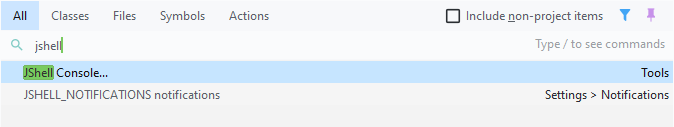
\includegraphics[width=0.5\textwidth]{img/Por_algo_se_empieza/idea64_search_everywhere.png}
      \caption{Resultado de \textit{Search Everywhere} para la búsqueda de \texttt{repl}.}
      \label{fig:idea64-search-everywhere}
    \end{figure}

    Ahora intenten reescribir el código del \cref{sec:Complicando_las_cosas} para ver cómo se siente 
    trabajar con un \textit{IDE} (reescríbanlo, no lo copien y peguen).
    Luego pueden ejecutar el código y ver el resultado en la consola presionando el botón 
    \enquote{\textit{play}} en la esquina superior izquierda de la pestaña.
    
    \begin{figure}[ht!]
      \centering
      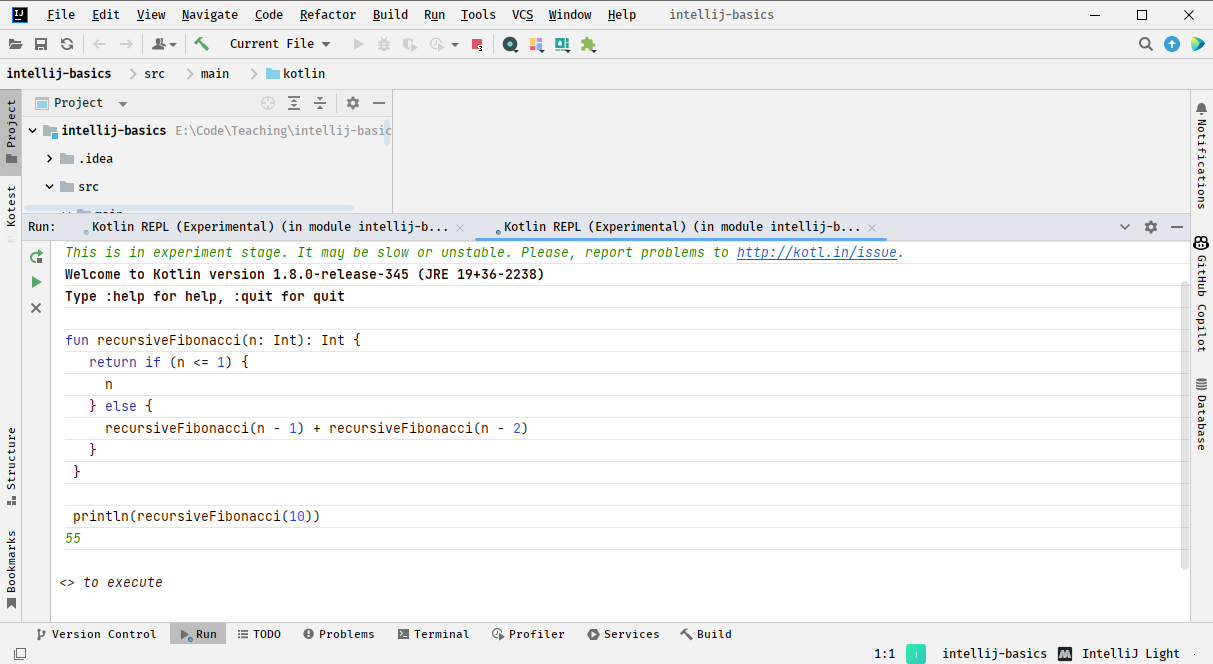
\includegraphics[width=0.9\textwidth]{img/Por_algo_se_empieza/idea64_fibonacci_repl.png}
      \caption{Ejemplo de uso de la \textit{consola REPL} en \textit{IntelliJ}.}
      \label{fig:idea64-fibonacci-repl}
    \end{figure}
  %endregion